\section{Tests des applications}

Tester l'application est une condition nécessaire si l'on veut s'assurer de sa qualité.
Les tests manuels par les développeurs ou les utilisateurs sont loin d'être suffisants : il existe bien trop de cas à vérifier.
Pour répondre à ce problème d'exhaustivité, il est possible de mettre en place des tests automatiques et programmables.
Aussi, on peut distinguer deux types de tests : les tests \emph{unitaires} et les tests \emph{fonctionnels}.



\subsection{Tests unitaires}

Pour expliquer ce qu'est ce premier type de tests, je m'en réfère à l'excellent article Wikipédia à ce sujet.~\cite{unit}

\begin{quotation}
Le test unitaire est un procédé permettant de s'assurer du fonctionnement correct d'une partie déterminée d'un logiciel ou d'une portion d'un programme (appelée \og unité \fg{} ou \og module \fg).

On écrit un test pour confronter une réalisation à sa spécification. Le test définit un critère d'arrêt (état ou sorties à l'issue de l'exécution) et permet de statuer sur le succès ou sur l'échec d'une vérification.
Grâce à la spécification, on est en mesure de faire correspondre un état d'entrée donné à un résultat ou à une sortie.
Le test permet de vérifier que la relation d'entrée/sortie donnée par la spécification est bel et bien réalisée.

Il s'agit pour le programmeur de tester un module, indépendamment du reste du programme, ceci afin de s'assurer qu'il répond aux spécifications fonctionnelles et qu'il fonctionne correctement en toutes circonstances.
Cette vérification est considérée comme essentielle, en particulier dans les applications critiques.
Elle s'accompagne couramment d'une vérification de la couverture de code (évaluation de la couverture structurelle), qui consiste à s'assurer que le test conduit à exécuter l'ensemble (ou une fraction déterminée) des instructions présentes dans le code à tester.

L'ensemble des tests unitaires doit être rejoué après une modification du code afin de vérifier qu'il n'y a pas de régressions (l'apparition de nouveaux dysfonctionnements).
\end{quotation}



\subsection{Tests fonctionnels}

Les tests fonctionnels diffèrent des tests unitaires du point de vue qu'ils vérifient les fonctionnalités de l'application.
Leur portée s'éloigne ainsi du code et devient globale à l'application.

Au niveau d'un site web, par exemple, un test fonctionnel consiste à naviguer à l'intérieur, en cliquant sur des liens, en remplissant des formulaires, ou encore en vérifiant si divers éléments d'une page sont bien présents.

Ce type de test prend tout son intérêt quand il s'agit de tester un cas d'utilisation typique d'une application par ses utilisateurs finaux.
En reproduisant un ensemble significatif des scénarios utilisateurs sous forme de tests fonctionnels, on peut alors s'assurer du bon fonctionnement global du programme, quels que soient les changement de code entrepris.



\subsection{Outils}

\subsubsection{Librairies de tests unitaires}

\paragraph{}
Chaque langage de programmation dispose de sa librairie pour rédiger des tests unitaires, si ce n'est plus.
Par exemple, on va trouver JUnit pour Java, PHPUnit ou Lime pour PHP, CppTest pour C++, etc.

\paragraph{}
La façon de rédiger des tests est souvent la même malgré les différences entre langages de programmation.
Pour une fonction, ce processus est répété pour chaque ensemble de paramètres d'entrée à tester :

\begin{enumerate}
	\item le contexte d'exécution est défini à travers des définition de variable est des appels de fonctions ;
	\item la fonction à tester unitairement est appelée, avec en entrée des paramètres choisis pour être des cas classiques ou des cas limites ;
	\item le retour de la fonction (voire même le déclenchement d'exception) est comparé à un résultat attendu issu des spécifications.
\end{enumerate}

Ainsi, chaque fonction à tester est exécutée plusieurs fois de suite avec des paramètres d'entrée différents afin de bien couvrir tous les cas.



\subsubsection{Selenium}

\paragraph{}
Selenium est un outil de tests fonctionnels pour les sites web.
Disponible sous la forme d'une extension pour le navigateur web Firefox, il enregistre l'enchaînement des liens cliqués pour naviguer de page en page.
Quand le test est joué, si une page du scénario ne s'affiche pas, on considère que c'est un échec.

Un autre test souvent utilisé est la vérification de la présence d'un texte sur une page.
C'est très pratique dans le cas où l'on veut vérifier la présence ou non d'erreurs après la soumission d'un formulaire, par exemple.

Enfin, le jeu de tests peut être sauvé dans un fichier afin de pouvoir être rejoué ultérieurement.

\paragraph{}
La \reffigure{pic-tests:selenium} montre une capture d'écran de Selenium.

\begin{figure}
	\centering
	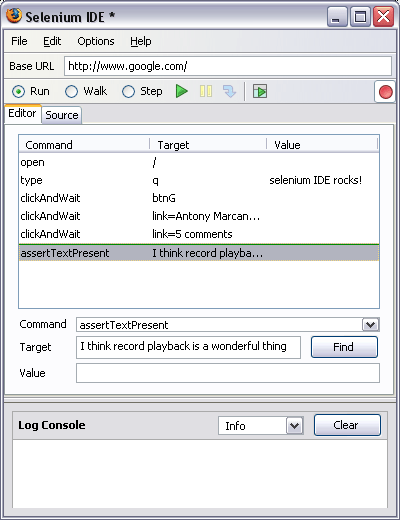
\includegraphics[width=7cm]{pic/selenium-ide}
	\caption{Selenium en action}
	\label{figure:pic-tests:selenium}
\end{figure}



\subsection{Missions}

\subsubsection{Formation Selenium chez Spir}

\paragraph{}
Spir est un éditeur de journaux de petites annonces qui édite aujourd'hui des sites \ainternet{} comme Top Annonces ou Logic Immo.
Pour améliorer son processus qualité, le client désire s'équiper d'un outil permettant de jouer automatiquement des tests fonctionnels.

\paragraph{}
Je me suis alors rendu dans leurs locaux avec \agulet{} pour leur présenter l'outil Selenium.
C'est une formation que j'ai préparée en amont moi-même et que nous avons présenté au client en duo.

